
\chapter{BIODATA PENULIS}

\begin{wrapfigure}{l}{0.3\textwidth}
	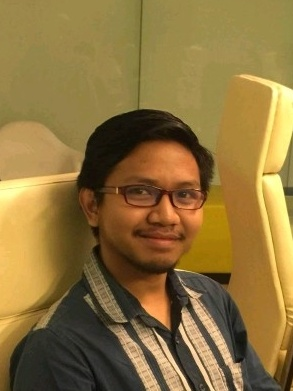
\includegraphics[height=0.25\textheight]{figures/william.jpg}
\end{wrapfigure}

Penulis bernama William Albertus Dembo, lahir di Sidoarjo pada tanggal 02 Februari 1997. Penulis telah menjalani masa pendidikan di Sekolah Dasar Katolik St Yustinus De Yacobis Krian pada tahun 2003 hingga 2009, Sekolah Menengah Pertama Katolik St Yustinus De Yacobis Krian pada tahung 2009 hingga 2012, dan Sekolah Menengah Atas Negeri 1 Krian pada tahun 2012 hingga 2015. Pada masa penulisan, penulis sedang menempuh masa studi S1 tahun ketiga di \jurusan, \fakultas, Institut Teknologi Sepuluh Nopember.

Selama masa studi S1, penulis memiliki ketertarikan yang dalam mengenai Algoritma dan Pemrograman, basis data, dan rancang bangun aplikasi situs web. Penulis pernah menjadi asisten dosen pada mata kuliah Dasar Pemrograman, Stuktur Data, dan Pemrograman Web. Dalam mengembangkan kemampuan yang dimiliki, penulis pernah menerima beberapa proyek untuk rancang bangun aplikasi web. Selain itu, penulis memiliki pengalaman magang di PT. Dwi Cermat Indonesia dan PT. Digital Otomotif Indonesia.

Di luar kesibukan akademik, penulis cukup aktif dalam organisasi baik dari dalam maupun luar jurusan. Penulis juga berkontribusi dalam kepanitiaan acara nasional selama 2 tahun. Selain itu, penulis pernah membantu kegiatan pelatihan nasional bagi peserta Olimpiade Komputer Indonesia pada tahun 2018 dan 2019. Penulis dapat dihubungi melalui surel di \href{mailto:w.albertusd@gmail.com}{w.albertusd@gmail.com}.